\documentclass[x11names,rgb]{standalone}
\usepackage{ifthen,calc}
\usepackage{tikz}
\usepackage{graphicx}
\usepackage{xfrac}
\usepackage{xstring}
\usepackage{siunitx}
\usetikzlibrary{%
  arrows,%
  automata,%
  shapes.misc,% wg. rounded rectangle
  shapes.arrows,%
  shapes.symbols,%
  shapes.gates.logic.US,%
  snakes,
  backgrounds,%
  calc,%
  math,%
  circuits,
  circuits.ee,
  circuits.ee.IEC,
  circuits.logic,
  circuits.logic.US,
  circuits.logic.IEC,
  chains,%
  fit,%
  matrix,%
  patterns,%
  positioning,% wg. " of "
  scopes,%
%  decorations.pathmorphing,% /pgf/decoration/random steps
  shadows%
}

\pgfkeys{
  /pighixxxpin/.is family, /pighixxxpin,
  connect color/.estore in     = \pighixxxConnectColor,      % connectors
  connect length/.estore in    = \pighixxxConnectLength,     % connectors
  connect linewidth/.estore in = \pighixxxConnectLinewidth,  % connectors
  angle/.estore in = \pighixxxAngle,
}

\pgfkeys{
  /pighixxxpin,
  default/.style =
  {%
    connect color = black,
    connect length = 2mm,
    connect linewidth = .3mm,
    angle = 0,
  }
}
\newcommand{\pighixxxpin}[3][]%
{%
  \pgfkeys{/pighixxxpin, default, #1}%
  \path(#2)coordinate(Ldummy);
  \pgfmathparse{-180+\pighixxxAngle}\edef\pighixxxNAngle{\pgfmathresult}
  \foreach[remember=\text as \lasttext (initially dummy)] \text/\tcol/\col/\w in {#3}%
  {%
    \ifthenelse{\pighixxxAngle > 90 \and \pighixxxAngle < 270}%
    {%
      \ifthenelse{\equal{\text}{}}{%
	    \edef\text{pighixxx}
	    \draw[draw=\pighixxxConnectColor,line width=\pighixxxConnectLinewidth]%
          (L\lasttext.west) -- ++(\pighixxxAngle:\pighixxxConnectLength)
		  -- ++(\pighixxxAngle:\w) coordinate(L\text);
	  }{%
        \draw[draw=\pighixxxConnectColor,line width=\pighixxxConnectLinewidth]%
          (L\lasttext.west) -- ++(\pighixxxAngle:\pighixxxConnectLength)%
          node[anchor=east,rotate=\pighixxxNAngle,text=\tcol,fill=\col,rounded corners=.5mm,inner sep=.5mm,draw=black,line width=.1mm,minimum width=\w]%
          (L\text){\ttfamily\tiny\text};
      }		
    }{%
      \ifthenelse{\equal{\text}{}}{%
	    \edef\text{pighixxx}
	    \draw[draw=\pighixxxConnectColor,line width=\pighixxxConnectLinewidth]%
          (L\lasttext.east) -- ++(\pighixxxAngle:\pighixxxConnectLength)
		  -- ++(\pighixxxAngle:\w) coordinate(L\text);
	  }{%
        \draw[draw=\pighixxxConnectColor,line width=\pighixxxConnectLinewidth]%
          (L\lasttext.east) -- ++(\pighixxxAngle:\pighixxxConnectLength)%
          node[anchor=west,rotate=\pighixxxAngle,text=\tcol,fill=\col,rounded corners=.5mm,inner sep=.5mm,draw=black,line width=.1mm,minimum width=\w]%
          (L\text){\ttfamily\tiny\text};
      }
	}
  }
}


\begin{document}
  \begin{tikzpicture}[x=1mm,y=1mm]
    % scale 2:1
    \path(0,.5) node[anchor=south,inner sep=0pt](im){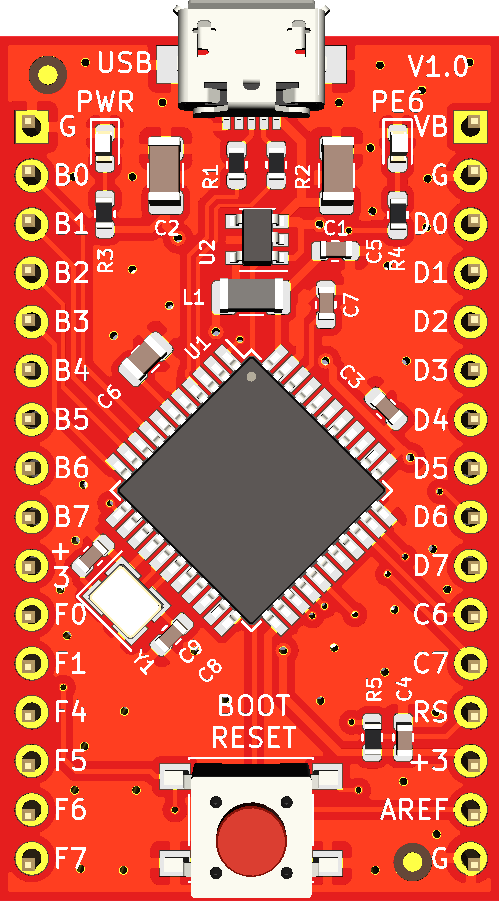
\includegraphics[width=26mm]{20210211_eduino_top}};
    \foreach[count=\cnt, evaluate=\cnt as \y using 43.5-\cnt*2.54] \i in {1,2,...,16}%
    {%
      \path(-13.2,\y) coordinate (pin\i);
      \path(pin\i)  ++(0,.5) node[anchor=south east,inner sep=0mm,text width=4mm,align=right,scale=.4,blue]{ \i};
    }
    \foreach[count=\cnt, evaluate=\cnt as \y using 0.32+\cnt*2.54] \i in {17,18,...,32}%
    {%
      \path(+13.2,\y) coordinate (pin\i);
      \path(pin\i) ++(0,.5) node[anchor=south west,inner sep=0mm,text width=4mm,align=left,scale=.4,blue]{ \i};
    }

    \pighixxxpin[angle=180]{pin1.south east}{GND/white/black/7mm}
    \pighixxxpin[angle=0]{pin17.south west}{GND/white/black/7mm}
    \pighixxxpin[angle=0]{pin31.south west}{GND/white/black/7mm}
    \pighixxxpin[angle=0]{pin32.south west}{+5 V/black/Red1/7mm}
    \pighixxxpin[angle=0]{pin19.south west}{+3.3 V/black/Red1/7mm}
    \pighixxxpin[angle=180]{pin10.south east}{+3.3 V/black/Red1/7mm}
    \pighixxxpin[angle=0]{pin18.south west}{AREF/black/SpringGreen3/7mm}
    \pighixxxpin[angle=0]{pin20.south west}{RESET/black/Gold1/7mm}

    \pighixxxpin[angle=180]{pin2.south east}{PB0/black/LightGoldenrod1/4mm,{17}/black/Magenta2/7mm,PCINT0/black/lightgray/8mm,SS/black/Turquoise1/8mm}
    \pighixxxpin[angle=180]{pin3.south east}{PB1/black/LightGoldenrod1/4mm,15/black/Magenta2/7mm,PCINT1/black/lightgray/8mm,SCK/black/Turquoise1/8mm}
    \pighixxxpin[angle=180]{pin4.south east}{PB2/black/LightGoldenrod1/4mm,16/black/Magenta2/7mm,PCINT2/black/lightgray/8mm,MOSI/black/Turquoise1/8mm,PDI/black/Gold1/8mm}
    \pighixxxpin[angle=180]{pin5.south east}{PB3/black/LightGoldenrod1/4mm,{14}/black/Magenta2/7mm,PCINT3/black/lightgray/8mm,MISO/black/Turquoise1/8mm,PDO/black/Gold1/8mm}
    \pighixxxpin[angle=180]{pin6.south east}{PB4/black/LightGoldenrod1/4mm,{8/A8}/black/Magenta2/7mm,PCINT4/black/lightgray/8mm,ADC11/black/SpringGreen3/8mm}
    \pighixxxpin[angle=180]{pin7.south east}{PB5/black/LightGoldenrod1/4mm,{9/A9}/black/Magenta2/7mm,PCINT5/black/lightgray/8mm,ADC12/black/SpringGreen3/8mm,OC1A/black/IndianRed1/8mm,{/OC4B}/black/IndianRed1/8mm}
    \pighixxxpin[angle=180]{pin8.south east}{PB6/black/LightGoldenrod1/4mm,{10/A10}/black/Magenta2/7mm,PCINT6/black/lightgray/8mm,ADC13/black/SpringGreen3/8mm,OC1B/black/IndianRed1/8mm,OC4B/black/IndianRed1/8mm}
    \pighixxxpin[angle=180]{pin9.south east}{PB7/black/LightGoldenrod1/4mm,11/black/Magenta2/7mm,PCINT7/black/lightgray/8mm,OC0A/black/IndianRed1/8mm,OC1C/black/IndianRed1/8mm,RTS/black/Aquamarine1/8mm}

    \pighixxxpin[angle=180]{pin11.south east}{PF0/black/LightGoldenrod1/4mm,{23/A5}/black/Magenta2/7mm,ADC0/black/SpringGreen3/8mm}
    \pighixxxpin[angle=180]{pin12.south east}{PF1/black/LightGoldenrod1/4mm,{22/A4}/black/Magenta2/7mm,ADC1/black/SpringGreen3/8mm}
    \pighixxxpin[angle=180]{pin13.south east}{PF4/black/LightGoldenrod1/4mm,{21/A3}/black/Magenta2/7mm,ADC4/black/SpringGreen3/8mm,TCK/black/Gold1/5mm}
    \pighixxxpin[angle=180]{pin14.south east}{PF5/black/LightGoldenrod1/4mm,{20/A2}/black/Magenta2/7mm,ADC5/black/SpringGreen3/8mm,TMS/black/Gold1/5mm}
    \pighixxxpin[angle=180]{pin15.south east}{PF6/black/LightGoldenrod1/4mm,{19/A1}/black/Magenta2/7mm,ADC6/black/SpringGreen3/8mm,TDO/black/Gold1/5mm}
    \pighixxxpin[angle=180]{pin16.south east}{PF7/black/LightGoldenrod1/4mm,{18/A0}/black/Magenta2/7mm,ADC7/black/SpringGreen3/8mm,TDI/black/Gold1/5mm}

    \pighixxxpin[angle=0]{pin22.south west}{PC6/black/LightGoldenrod1/4mm,{5}/black/Magenta2/7mm,OC3A/black/IndianRed1/8mm,{/OC4A}/black/IndianRed1/8mm}
    \pighixxxpin[angle=0]{pin21.south west}{PC7/black/LightGoldenrod1/4mm,{13}/black/Magenta2/7mm,CLKO/black/Gold1/8mm,OC4A/black/IndianRed1/8mm,ICP3/black/Thistle2/8mm}

    \pighixxxpin[angle=0]{pin30.south west}{PD0/black/LightGoldenrod1/4mm,{3}/black/Magenta2/7mm,INT0/black/lightgray/8mm,SCL/black/SteelBlue1/5mm}
    \pighixxxpin[angle=0]{pin29.south west}{PD1/black/LightGoldenrod1/4mm,{2}/black/Magenta2/7mm,INT1/black/lightgray/8mm,SDA/black/SteelBlue1/5mm}
    \pighixxxpin[angle=0]{pin28.south west}{PD2/black/LightGoldenrod1/4mm,{0}/black/Magenta2/7mm,INT2/black/lightgray/8mm,RXD1/black/Aquamarine1/8mm}
    \pighixxxpin[angle=0]{pin27.south west}{PD3/black/LightGoldenrod1/4mm,{1}/black/Magenta2/7mm,INT3/black/lightgray/8mm,TXD1/black/Aquamarine1/8mm}
    \pighixxxpin[angle=0]{pin26.south west}{PD4/black/LightGoldenrod1/4mm,{4/A6}/black/Magenta2/7mm,ICP1/black/Thistle2/8mm,ADC8/black/SpringGreen3/8mm}
    \pighixxxpin[angle=0]{pin25.south west}{PD5/black/LightGoldenrod1/4mm,{TLED}/black/Magenta2/7mm,XCK1/black/Aquamarine1/8mm,CTS/black/Aquamarine1/8mm}
    \pighixxxpin[angle=0]{pin24.south west}{PD6/black/LightGoldenrod1/4mm,{12/A11}/black/Magenta2/7mm,T1/black/Thistle2/8mm,{/OC4D}/black/IndianRed1/8mm,ADC9/black/SpringGreen3/8mm}
    \pighixxxpin[angle=0]{pin23.south west}{PD7/black/LightGoldenrod1/4mm,{6/A7}/black/Magenta2/7mm,T0/black/Thistle2/8mm,OC4D/black/IndianRed1/8mm,ADC10/black/SpringGreen3/8mm}

    \path (-75,18) coordinate (legend);
    \fill [AntiqueWhite1,rounded corners = 1mm] (legend) rectangle ++(28,-19);

    \path ($(legend) + (1, -2)$) node[anchor=west,draw=black,line width=.1mm,fill=Red1,minimum width=3mm,minimum height=1.5mm,inner sep=0pt](power){};
    \path (power.east) node[anchor=west,inner sep=2pt]{\sffamily\slshape\tiny power};

    \path ($(legend) + (16, -2)$) node[anchor=west,draw=black,line width=.1mm,fill=black,text=white,minimum width=3mm,minimum height=1.5mm,inner sep=0pt](int){};
    \path (int.east) node[anchor=west,inner sep=2pt]{\sffamily\slshape\tiny GND};

    \path ($(legend) + (1, -17)$) node[anchor=west,draw=black,line width=.1mm,fill=Gold1,text=black,minimum width=3mm,minimum height=1.5mm,inner sep=0pt](int){};
    \path (int.east) node[anchor=west,inner sep=2pt]{\sffamily\slshape\tiny ctrl \& JTAG};

    \path ($(legend) + (16, -17)$) node[anchor=west,draw=black,line width=.1mm,fill=Magenta2,text=black,minimum width=3mm,minimum height=1.5mm,inner sep=0pt](int){};
    \path (int.east) node[anchor=west,inner sep=2pt]{\sffamily\slshape\tiny Arduino};

    \path ($(legend) + (1, -5)$) node[anchor=west,draw=black,line width=.1mm,fill=LightGoldenrod1,minimum width=3mm,minimum height=1.5mm,inner sep=0pt](gpio){};
    \path (gpio.east) node[anchor=west,inner sep=2pt]{\sffamily\slshape\tiny GPIO};

    \path ($(legend) + (1, -8)$) node[anchor=west,draw=black,line width=.1mm,fill=SpringGreen3,minimum width=3mm,minimum height=1.5mm,inner sep=0pt](adc){};
    \path (adc.east) node[anchor=west,inner sep=2pt]{\sffamily\slshape\tiny ADC};

    \path ($(legend) + (16, -5)$) node[anchor=west,draw=black,line width=.1mm,fill=Aquamarine1,minimum width=3mm,minimum height=1.5mm,inner sep=0pt](uart){};
    \path (uart.east) node[anchor=west,inner sep=2pt]{\sffamily\slshape\tiny UART};

    \path ($(legend) + (16, -8)$) node[anchor=west,draw=black,line width=.1mm,fill=Turquoise1,minimum width=3mm,minimum height=1.5mm,inner sep=0pt](spi){};
    \path (spi.east) node[anchor=west,inner sep=2pt]{\sffamily\slshape\tiny SPI};

    \path ($(legend) + (16, -11)$) node[anchor=west,draw=black,line width=.1mm,fill=SteelBlue1,minimum width=3mm,minimum height=1.5mm,inner sep=0pt](i2c){};
    \path (i2c.east) node[anchor=west,inner sep=2pt]{\sffamily\slshape\tiny I2C};

    \path ($(legend) + (1, -11)$) node[anchor=west,draw=black,line width=.1mm,fill=Thistle2,minimum width=3mm,minimum height=1.5mm,inner sep=0pt](timer){};
    \path (timer.east) node[anchor=west,inner sep=2pt]{\sffamily\slshape\tiny timers};

    \path ($(legend) + (1, -14)$) node[anchor=west,draw=black,line width=.1mm,fill=IndianRed1,minimum width=3mm,minimum height=1.5mm,inner sep=0pt](timer){};
    \path (timer.east) node[anchor=west,inner sep=2pt]{\sffamily\slshape\tiny PWM};

    \path ($(legend) + (16, -14)$) node[anchor=west,draw=black,line width=.1mm,fill=lightgray,minimum width=3mm,minimum height=1.5mm,inner sep=0pt](int){};
    \path (int.east) node[anchor=west,inner sep=2pt]{\sffamily\slshape\tiny interrupts};


    \path (25,10) coordinate (legend2);
    \fill [AntiqueWhite1,rounded corners = 1mm] (legend2) rectangle ++(36,-11);
    \path ($(legend2.north west)+(1.5,-1.5)$) node[anchor=north west, text width=68mm, inner sep=0pt,scale=.5]%
    {Arduino reference is for Arduino Leonardo and compatible units.\newline
    Arduino digital pin 7 is connected to the right LED, not available on the pinheader.};

  \end{tikzpicture}

\end{document}
